\documentclass[10pt]{paper}\usepackage[]{graphicx}\usepackage[]{color}
%% maxwidth is the original width if it is less than linewidth
%% otherwise use linewidth (to make sure the graphics do not exceed the margin)
\makeatletter
\def\maxwidth{ %
  \ifdim\Gin@nat@width>\linewidth
    \linewidth
  \else
    \Gin@nat@width
  \fi
}
\makeatother

\definecolor{fgcolor}{rgb}{0.345, 0.345, 0.345}
\newcommand{\hlnum}[1]{\textcolor[rgb]{0.686,0.059,0.569}{#1}}%
\newcommand{\hlstr}[1]{\textcolor[rgb]{0.192,0.494,0.8}{#1}}%
\newcommand{\hlcom}[1]{\textcolor[rgb]{0.678,0.584,0.686}{\textit{#1}}}%
\newcommand{\hlopt}[1]{\textcolor[rgb]{0,0,0}{#1}}%
\newcommand{\hlstd}[1]{\textcolor[rgb]{0.345,0.345,0.345}{#1}}%
\newcommand{\hlkwa}[1]{\textcolor[rgb]{0.161,0.373,0.58}{\textbf{#1}}}%
\newcommand{\hlkwb}[1]{\textcolor[rgb]{0.69,0.353,0.396}{#1}}%
\newcommand{\hlkwc}[1]{\textcolor[rgb]{0.333,0.667,0.333}{#1}}%
\newcommand{\hlkwd}[1]{\textcolor[rgb]{0.737,0.353,0.396}{\textbf{#1}}}%
\let\hlipl\hlkwb

\usepackage{framed}
\makeatletter
\newenvironment{kframe}{%
 \def\at@end@of@kframe{}%
 \ifinner\ifhmode%
  \def\at@end@of@kframe{\end{minipage}}%
  \begin{minipage}{\columnwidth}%
 \fi\fi%
 \def\FrameCommand##1{\hskip\@totalleftmargin \hskip-\fboxsep
 \colorbox{shadecolor}{##1}\hskip-\fboxsep
     % There is no \\@totalrightmargin, so:
     \hskip-\linewidth \hskip-\@totalleftmargin \hskip\columnwidth}%
 \MakeFramed {\advance\hsize-\width
   \@totalleftmargin\z@ \linewidth\hsize
   \@setminipage}}%
 {\par\unskip\endMakeFramed%
 \at@end@of@kframe}
\makeatother

\definecolor{shadecolor}{rgb}{.97, .97, .97}
\definecolor{messagecolor}{rgb}{0, 0, 0}
\definecolor{warningcolor}{rgb}{1, 0, 1}
\definecolor{errorcolor}{rgb}{1, 0, 0}
\newenvironment{knitrout}{}{} % an empty environment to be redefined in TeX

\usepackage{alltt}

\usepackage{amsmath}
\usepackage{listings}
\usepackage{color}
\usepackage{amssymb}
\usepackage{float}
\usepackage[margin=.5in]{geometry}
\usepackage{graphicx}
\IfFileExists{upquote.sty}{\usepackage{upquote}}{}
\begin{document}
\section*{Question 1}

\subsection*{a}

\begin{knitrout}
\definecolor{shadecolor}{rgb}{0.969, 0.969, 0.969}\color{fgcolor}\begin{kframe}
\begin{alltt}
\hlstd{data} \hlkwb{<-} \hlkwd{read.table}\hlstd{(} \hlstr{"Galton.dat"} \hlstd{)}

\hlstd{sons} \hlkwb{<-} \hlstd{data[data}\hlopt{$}\hlstd{V4}\hlopt{==}\hlnum{1}\hlstd{,]}
\hlstd{daughters} \hlkwb{<-} \hlstd{data[data}\hlopt{$}\hlstd{V4}\hlopt{==}\hlnum{0}\hlstd{,]}
\hlstd{fathers} \hlkwb{<-} \hlkwd{unique}\hlstd{( data[,}\hlnum{1}\hlopt{:}\hlnum{2}\hlstd{])}


\hlkwd{summary}\hlstd{(sons}\hlopt{$}\hlstd{V5)}
\end{alltt}
\begin{verbatim}
##    Min. 1st Qu.  Median    Mean 3rd Qu.    Max. 
##   0.000   7.500   9.200   9.234  11.000  19.000
\end{verbatim}
\begin{alltt}
\hlkwd{sd}\hlstd{( sons}\hlopt{$}\hlstd{V5)}
\end{alltt}
\begin{verbatim}
## [1] 2.623688
\end{verbatim}
\begin{alltt}
\hlkwd{max}\hlstd{( sons}\hlopt{$}\hlstd{V5 )} \hlopt{-} \hlkwd{min}\hlstd{( sons}\hlopt{$}\hlstd{V5 )}
\end{alltt}
\begin{verbatim}
## [1] 19
\end{verbatim}
\begin{alltt}
\hlkwd{IQR}\hlstd{( sons}\hlopt{$}\hlstd{V5 )}
\end{alltt}
\begin{verbatim}
## [1] 3.5
\end{verbatim}
\begin{alltt}
\hlkwd{summary}\hlstd{( daughters}\hlopt{$}\hlstd{V5 )}
\end{alltt}
\begin{verbatim}
##    Min. 1st Qu.  Median    Mean 3rd Qu.    Max. 
##  -4.000   2.500   4.000   4.103   5.500  10.500
\end{verbatim}
\begin{alltt}
\hlkwd{sd}\hlstd{( daughters}\hlopt{$}\hlstd{V5)}
\end{alltt}
\begin{verbatim}
## [1] 2.356053
\end{verbatim}
\begin{alltt}
\hlkwd{max}\hlstd{( daughters}\hlopt{$}\hlstd{V5 )} \hlopt{-} \hlkwd{min}\hlstd{( daughters}\hlopt{$}\hlstd{V5 )}
\end{alltt}
\begin{verbatim}
## [1] 14.5
\end{verbatim}
\begin{alltt}
\hlkwd{IQR}\hlstd{( daughters}\hlopt{$}\hlstd{V5 )}
\end{alltt}
\begin{verbatim}
## [1] 3
\end{verbatim}
\end{kframe}
\end{knitrout}

Both fathers and mothers that have large families would be over-represented by
the data, since there is one row per offspring. Parents of families that had
more than one son or daughter would appear more than once, leading to them being
mis-represented. This problem can be rectified with the unique function that was
applied to the variable \it{fathers}.

\subsection*{b}
\begin{knitrout}
\definecolor{shadecolor}{rgb}{0.969, 0.969, 0.969}\color{fgcolor}\begin{kframe}
\begin{alltt}
\hlkwd{plot}\hlstd{(} \hlkwc{x}\hlstd{=sons}\hlopt{$}\hlstd{V2,}\hlkwc{y}\hlstd{=sons}\hlopt{$}\hlstd{V5,} \hlkwc{xlab}\hlstd{=}\hlstr{"Fathers"}\hlstd{,} \hlkwc{ylab}\hlstd{=}\hlstr{"Sons"}\hlstd{)}
\end{alltt}
\end{kframe}
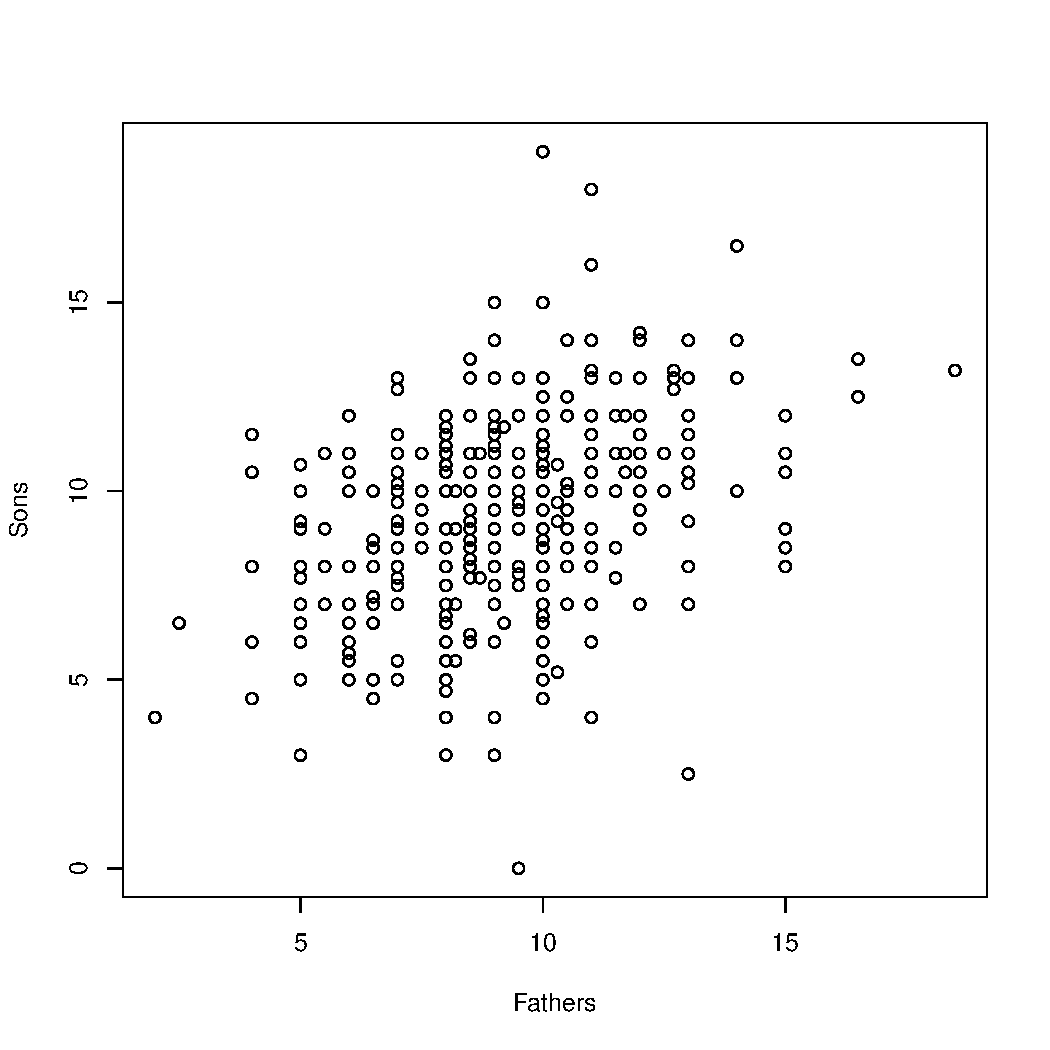
\includegraphics[width=\maxwidth]{figure/OneB-1} 

\end{knitrout}

\section*{Question 2}

\subsection*{a}

\begin{knitrout}
\definecolor{shadecolor}{rgb}{0.969, 0.969, 0.969}\color{fgcolor}\begin{kframe}
\begin{alltt}
\hlstd{GenerateEDF} \hlkwb{<-} \hlkwa{function}\hlstd{(} \hlkwc{depth}\hlstd{,} \hlkwc{frame}\hlstd{,} \hlkwc{start}\hlstd{,} \hlkwc{end} \hlstd{)\{}
    \hlstd{EDF} \hlkwb{<-} \hlkwd{numeric}\hlstd{( (end}\hlopt{-}\hlstd{start)}\hlopt{*}\hlstd{depth )}
    \hlstd{i} \hlkwb{<-} \hlnum{0}
    \hlkwa{for}\hlstd{( i} \hlkwa{in} \hlnum{1}\hlopt{:}\hlkwd{length}\hlstd{( EDF ))\{}
        \hlstd{EDF[i]} \hlkwb{<-} \hlkwd{length}\hlstd{( frame[frame}\hlopt{<=}\hlstd{(start}\hlopt{+}\hlstd{(i}\hlopt{/}\hlstd{depth))] )} \hlopt{/} \hlkwd{length}\hlstd{( frame )}
    \hlstd{\}}
    \hlstd{EDF}
\hlstd{\}}
\hlstd{depth} \hlkwb{<-}  \hlnum{100}

\hlstd{start} \hlkwb{<-} \hlkwd{min}\hlstd{( sons}\hlopt{$}\hlstd{V5, daughters}\hlopt{$}\hlstd{V5 )}
\hlstd{end} \hlkwb{<-} \hlkwd{max}\hlstd{( sons}\hlopt{$}\hlstd{V5, daughters}\hlopt{$}\hlstd{V5 )}


\hlstd{sonEDF} \hlkwb{<-} \hlkwd{GenerateEDF}\hlstd{( depth, sons}\hlopt{$}\hlstd{V5, start, end )}
\hlstd{daughterEDF} \hlkwb{<-} \hlkwd{GenerateEDF}\hlstd{( depth, daughters}\hlopt{$}\hlstd{V5, start, end )}

\hlstd{inches} \hlkwb{<-}  \hlkwd{numeric}\hlstd{( (end}\hlopt{-}\hlstd{start)}\hlopt{*}\hlstd{depth )}
\hlkwa{for}\hlstd{( i} \hlkwa{in} \hlnum{1}\hlopt{:}\hlkwd{length}\hlstd{(inches))\{}
    \hlstd{inches[i]} \hlkwb{<-} \hlstd{start} \hlopt{+} \hlstd{i}\hlopt{/}\hlstd{depth} \hlopt{+} \hlnum{60}
\hlstd{\}}

\hlkwd{plot}\hlstd{(} \hlkwc{x}\hlstd{=inches,} \hlkwc{y}\hlstd{=sonEDF,} \hlkwc{type}\hlstd{=}\hlstr{"l"}\hlstd{,} \hlkwc{col}\hlstd{=}\hlstr{"blue"} \hlstd{)}
\hlkwd{lines}\hlstd{(} \hlkwc{x}\hlstd{=inches,}\hlkwc{y}\hlstd{=daughterEDF,} \hlkwc{col}\hlstd{=}\hlstr{"pink"}\hlstd{)}
\hlkwd{legend}\hlstd{(} \hlnum{70}\hlstd{,}\hlnum{.2}\hlstd{,} \hlkwc{legend}\hlstd{=}\hlkwd{c}\hlstd{(}\hlstr{"Sons"}\hlstd{,}\hlstr{"Daughters"}\hlstd{),} \hlkwc{lty} \hlstd{=} \hlkwd{c}\hlstd{(}\hlnum{1}\hlstd{,}\hlnum{1}\hlstd{) ,} \hlkwc{col}\hlstd{=}\hlkwd{c}\hlstd{(}\hlstr{"blue"}\hlstd{,}\hlstr{"pink"}\hlstd{))}
\end{alltt}
\end{kframe}
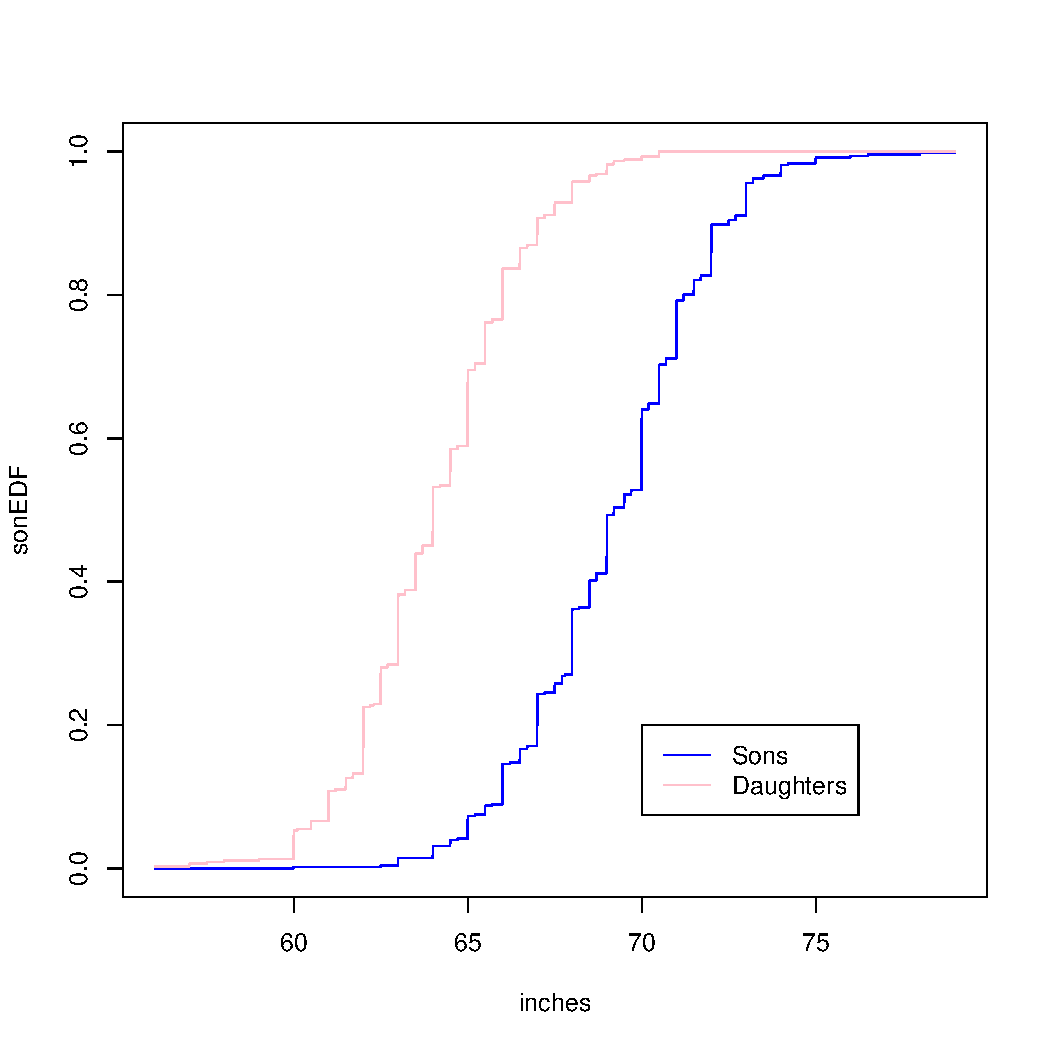
\includegraphics[width=\maxwidth]{figure/TwoA-1} 

\end{knitrout}

\subsection*{b}

\begin{knitrout}
\definecolor{shadecolor}{rgb}{0.969, 0.969, 0.969}\color{fgcolor}\begin{kframe}
\begin{alltt}
\hlstd{fatherEDF} \hlkwb{<-} \hlkwd{GenerateEDF}\hlstd{( depth, fathers}\hlopt{$}\hlstd{V2, start, end )}

\hlkwd{plot}\hlstd{(} \hlkwc{x} \hlstd{= inches,} \hlkwc{y}\hlstd{=fatherEDF,} \hlkwc{type}\hlstd{=}\hlstr{"l"}\hlstd{,} \hlkwc{col}\hlstd{=}\hlstr{"blue"} \hlstd{)}
\hlkwd{lines}\hlstd{(}\hlkwc{x}\hlstd{=inches,}\hlkwc{y}\hlstd{=sonEDF,}\hlkwc{col}\hlstd{=}\hlstr{"red"}\hlstd{)}
\hlkwd{legend}\hlstd{(} \hlnum{60}\hlstd{,}\hlnum{1}\hlstd{,} \hlkwc{legend}\hlstd{=}\hlkwd{c}\hlstd{(}\hlstr{"Fathers"}\hlstd{,}\hlstr{"Sons"}\hlstd{),} \hlkwc{lty} \hlstd{=} \hlkwd{c}\hlstd{(}\hlnum{1}\hlstd{,}\hlnum{1}\hlstd{) ,} \hlkwc{col}\hlstd{=}\hlkwd{c}\hlstd{(}\hlstr{"blue"}\hlstd{,}\hlstr{"red"}\hlstd{))}
\end{alltt}
\end{kframe}
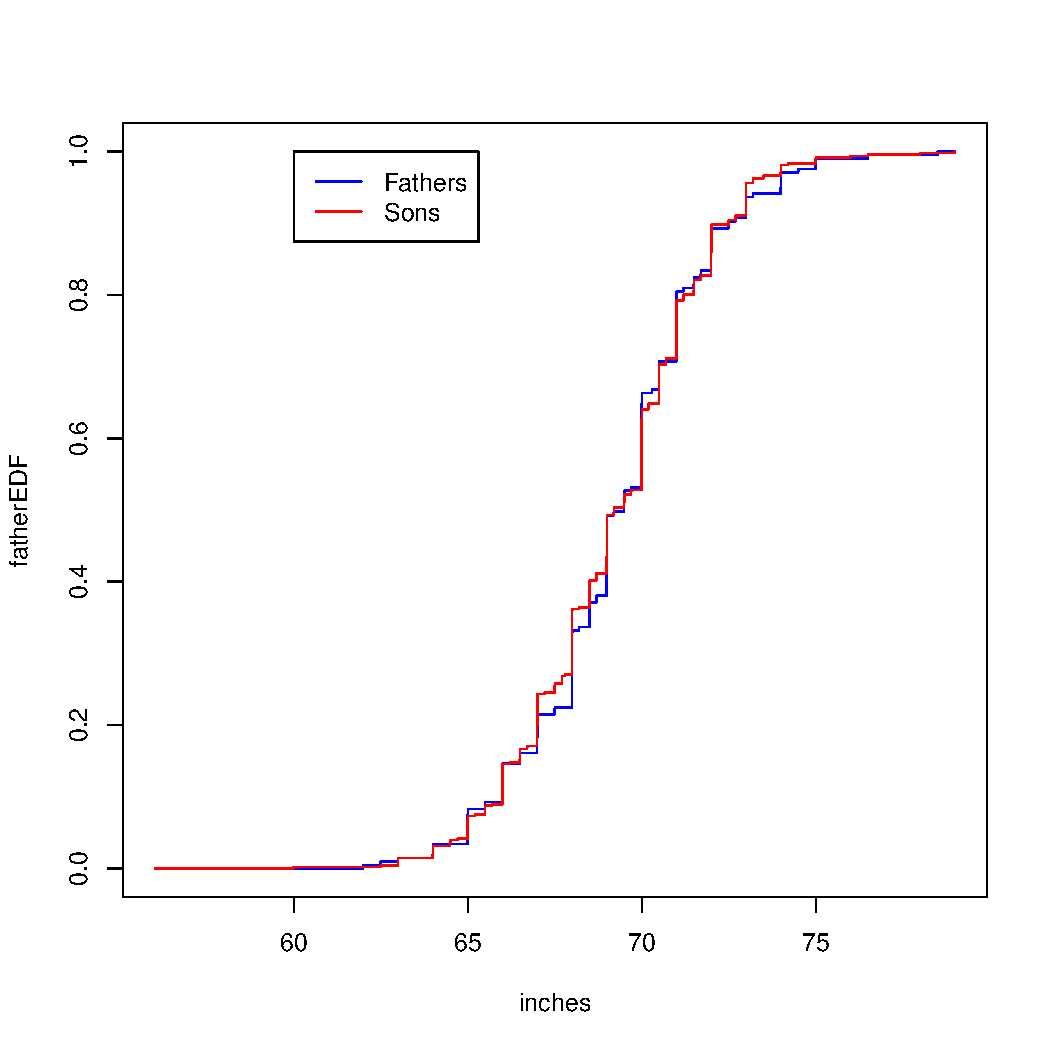
\includegraphics[width=\maxwidth]{figure/TwoB-1} 

\end{knitrout}

\section*{Question 3.}

\begin{knitrout}
\definecolor{shadecolor}{rgb}{0.969, 0.969, 0.969}\color{fgcolor}\begin{kframe}
\begin{alltt}
\hlstd{depth} \hlkwb{<-}  \hlnum{100}


\hlstd{NormalKernal} \hlkwb{<-} \hlkwa{function}\hlstd{(} \hlkwc{u} \hlstd{)\{}
    \hlstd{(}\hlnum{1}\hlopt{/}\hlkwd{sqrt}\hlstd{(} \hlnum{2}\hlopt{*}\hlstd{pi))}\hlopt{*}\hlkwd{exp}\hlstd{( (}\hlopt{-}\hlnum{1}\hlopt{*}\hlstd{u}\hlopt{^}\hlnum{2}\hlstd{)}\hlopt{/}\hlnum{2.0} \hlstd{)}
\hlstd{\}}

\hlstd{GenerateKernalSmoothHistogram} \hlkwb{<-} \hlkwa{function}\hlstd{(} \hlkwc{depth}\hlstd{,} \hlkwc{frame}\hlstd{,} \hlkwc{start}\hlstd{,} \hlkwc{end}\hlstd{,} \hlkwc{kernal} \hlstd{)\{}
    \hlstd{kSmooth} \hlkwb{<-} \hlkwd{numeric}\hlstd{( (end}\hlopt{-}\hlstd{start)}\hlopt{*}\hlstd{depth )}
    \hlstd{i} \hlkwb{<-} \hlnum{0}
    \hlstd{h} \hlkwb{<-} \hlnum{1.06}\hlopt{*}\hlkwd{sd}\hlstd{(frame)}\hlopt{*}\hlkwd{as.numeric}\hlstd{(}\hlkwd{length}\hlstd{(frame))}\hlopt{^}\hlstd{(}\hlopt{-}\hlnum{1.0}\hlopt{/}\hlnum{5.0}\hlstd{)}
    \hlkwa{for}\hlstd{( i} \hlkwa{in} \hlnum{1}\hlopt{:}\hlkwd{length}\hlstd{(kSmooth) )\{}
        \hlstd{kSmooth[i]} \hlkwb{<-} \hlnum{0}
        \hlstd{y} \hlkwb{<-} \hlstd{(start}\hlopt{+}\hlstd{(i}\hlopt{/}\hlstd{depth))}
        \hlkwa{for}\hlstd{( j} \hlkwa{in} \hlnum{1}\hlopt{:}\hlkwd{length}\hlstd{(frame))\{}
            \hlstd{kSmooth[i]} \hlkwb{<-} \hlstd{kSmooth[i]} \hlopt{+} \hlkwd{kernal}\hlstd{( (y} \hlopt{-} \hlstd{frame[j])}\hlopt{/}\hlstd{h )}
        \hlstd{\}}
        \hlstd{kSmooth[i]} \hlkwb{<-} \hlstd{kSmooth[i]} \hlopt{/} \hlstd{(}\hlkwd{length}\hlstd{(frame)}\hlopt{*}\hlstd{h)}
    \hlstd{\}}
    \hlstd{kSmooth}
\hlstd{\}}

\hlstd{start} \hlkwb{<-} \hlkwd{min}\hlstd{( sons}\hlopt{$}\hlstd{V5, daughters}\hlopt{$}\hlstd{V5 )} \hlopt{-} \hlnum{10}
\hlstd{end} \hlkwb{<-} \hlkwd{max}\hlstd{( sons}\hlopt{$}\hlstd{V5, daughters}\hlopt{$}\hlstd{V5 )} \hlopt{+} \hlnum{10}

\hlstd{sonHist} \hlkwb{<-} \hlkwd{GenerateKernalSmoothHistogram}\hlstd{( depth, sons}\hlopt{$}\hlstd{V5, start, end, NormalKernal )}
\hlstd{daughterHist} \hlkwb{<-} \hlkwd{GenerateKernalSmoothHistogram}\hlstd{( depth, daughters}\hlopt{$}\hlstd{V5, start, end, NormalKernal )}
\hlstd{fatherHist} \hlkwb{<-} \hlkwd{GenerateKernalSmoothHistogram}\hlstd{( depth, fathers}\hlopt{$}\hlstd{V2, start, end, NormalKernal )}
\hlstd{inches} \hlkwb{<-}  \hlkwd{numeric}\hlstd{( (end}\hlopt{-}\hlstd{start)}\hlopt{*}\hlstd{depth )}
\hlkwa{for}\hlstd{( i} \hlkwa{in} \hlnum{1}\hlopt{:}\hlkwd{length}\hlstd{(inches))\{}
    \hlstd{inches[i]} \hlkwb{<-} \hlstd{start} \hlopt{+} \hlstd{i}\hlopt{/}\hlstd{depth} \hlopt{+} \hlnum{60}
\hlstd{\}}

\hlkwd{plot}\hlstd{(} \hlkwc{x}\hlstd{=inches,}\hlkwc{y}\hlstd{=fatherHist,} \hlkwc{type}\hlstd{=}\hlstr{"l"}\hlstd{,} \hlkwc{col}\hlstd{=}\hlstr{"blue"} \hlstd{)}
\hlkwd{lines}\hlstd{(}\hlkwc{x}\hlstd{=inches,}\hlkwc{y}\hlstd{=sonHist,} \hlkwc{col}\hlstd{=}\hlstr{"red"} \hlstd{)}
\hlkwd{legend}\hlstd{(} \hlnum{80}\hlstd{,}\hlnum{.15}\hlstd{,} \hlkwc{legend}\hlstd{=}\hlkwd{c}\hlstd{(}\hlstr{"Fathers"}\hlstd{,}\hlstr{"Sons"}\hlstd{),} \hlkwc{lty} \hlstd{=} \hlkwd{c}\hlstd{(}\hlnum{1}\hlstd{,}\hlnum{1}\hlstd{) ,} \hlkwc{col}\hlstd{=}\hlkwd{c}\hlstd{(}\hlstr{"blue"}\hlstd{,}\hlstr{"red"}\hlstd{))}
\end{alltt}
\end{kframe}
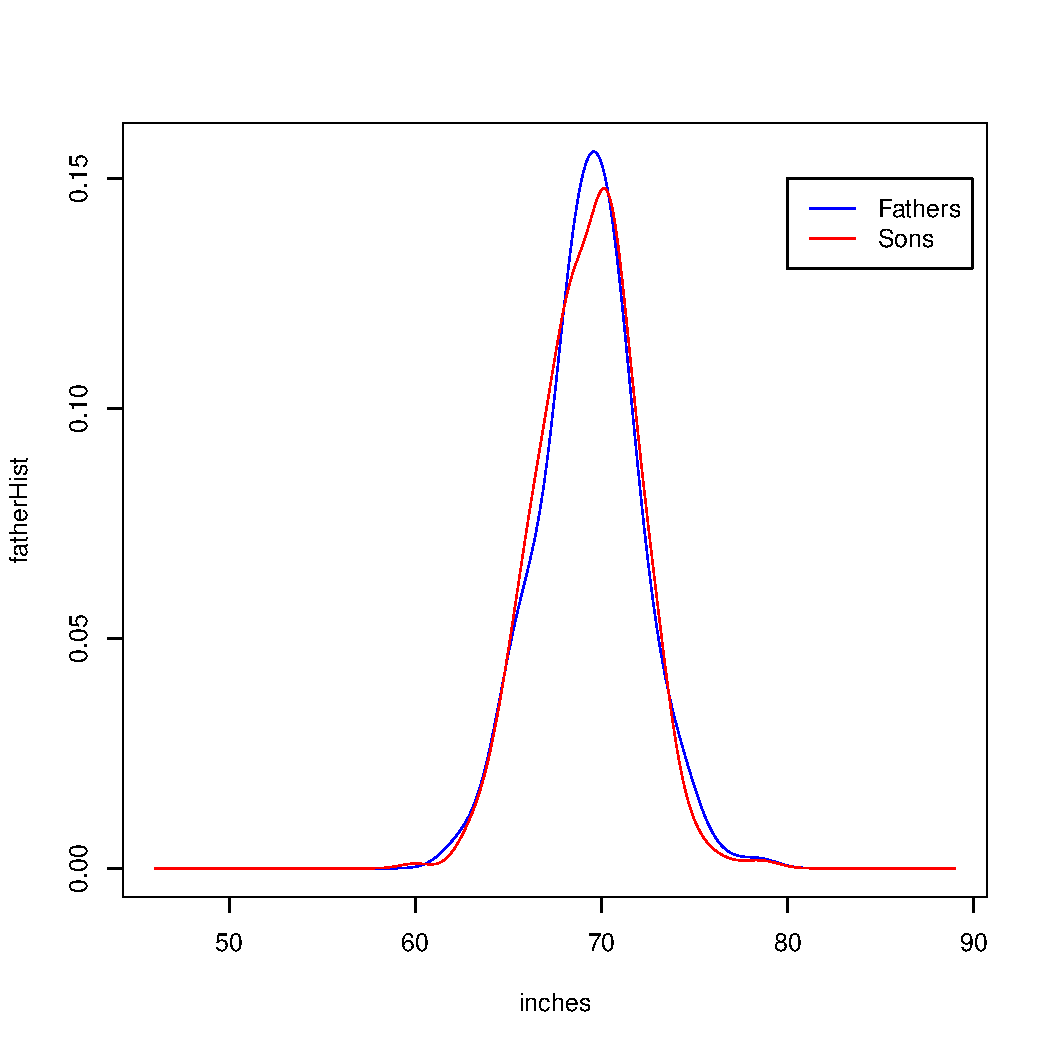
\includegraphics[width=6in]{figure/ThreeA-1} 

\end{knitrout}

\end{document}
